\documentclass[a4paper,10pt]{article}
\usepackage[utf8]{inputenc}
\usepackage{xspace}
\usepackage{graphicx,graphics} 


%opening
\title{Algorithmic model for N-GREEN optical ring}




\begin{document}

\maketitle

\section*{Definitions, model}
We consider an optical ring composed of $k$ nodes.
We are in a discrete time Model: The time is split in $N$ slot, rotating to the following position each time step $t$. The number of slots is given by the length of the ring, and the time step $t$ is the switching granularity. 
\begin{center}   

      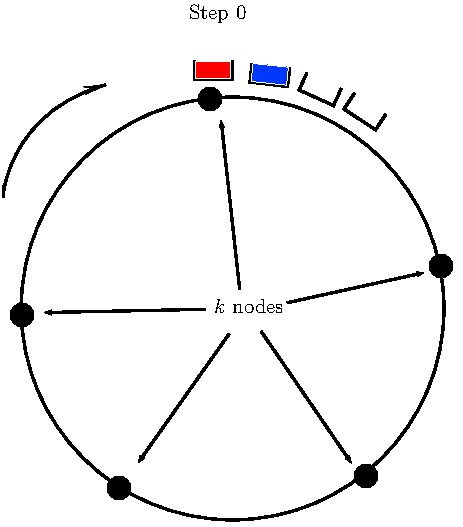
\includegraphics[scale=0.5]{anneau1.pdf}
      \hspace{3cm}
      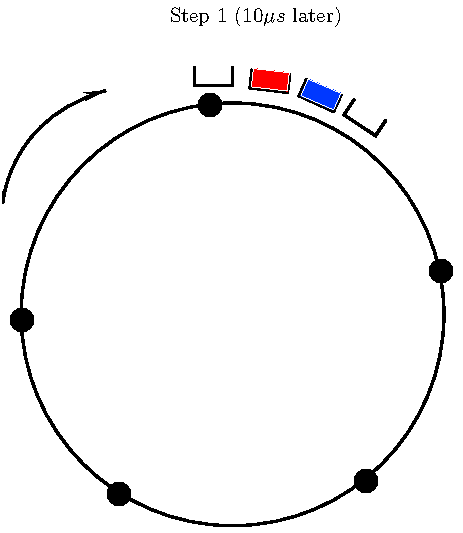
\includegraphics[scale=0.5]{anneau2.pdf}
  
\end{center}

We consider a ring as a graph model. The weight of the arcs is the time taken by a slot to travel the link, i.e. a multiple of $t$. The sum of all the weight of the arcs in the graph is equal to $t.N$.

\section*{Periodic process}
We define a set $\cal C$ of couple of vertices $(u,v) \in V$. Between each couple of $\cal C$, the following periodic process of period $P$ ($P$ is a multiple of $N$) is observed.
\begin{enumerate}
 \item The node $u$ receives (from an external way) some latency critical data addressed to $v$.
 \item Those data are transferred to $v$ through the ring .
 \item After reception and computing of the message, the node $v$ sends an answer to $u$.
\end{enumerate}
 This periodic process has a critical end to end latency, thus a messages has to be the less buffered as possible before being send in the ring.
 
\section*{Sending policy}
In the studied model, the ring has a {\bf broadcast and select} policy: when a node sends some data in a slot, this slot is {\em taken} by this node for an entire ride of the ring. This means that every nodes of the ring can collect the information addressed to it, but it does not delete the data in the slot. The slot is fully cleared by the node that sent it, when it came back after a ride of the ring.

Thus, a node has to wait for a free slot before sending some data in the ring. To avoid overloading the ring, a node sends some data only if some criteria  are satisfied.
We define by $Q$ the size of the buffer of a node, $\alpha$ the {\em minimum load} of the buffer, $0 \leq  \alpha \leq 1$, and $\delta$ the {\em maximum delay}.

The node sends some data in a slot if:
\begin{itemize}
 \item The amount of data $q$ in the buffer is greater than $\alpha . Q$,
 \item or the older data in the buffer is waiting for more than $\delta$.
\end{itemize}

In C-RAN context, this amount of data $q$ contains two kinds of data: the latency critical flow coming from RRH or BBU, and an other flow, called {\em best effort}.

We can consider two buffers containing $x$ and $y$ amount of data, respectively for the C-RAN flow and the best effort flow.
The data in the first buffer are inserted first in the buffer of the node, and comes periodically in regard of the period $P$. 
The best effort data comes more randomly (can be modelled by a Poisson distribution, for example), and are inserted in the buffer if $x = 0$.

\begin{center}   

      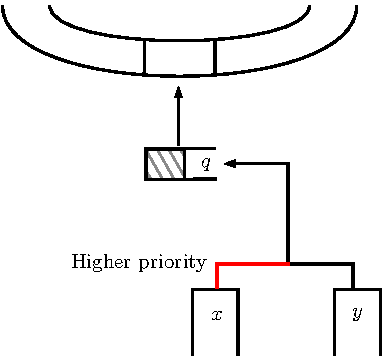
\includegraphics[scale=0.7]{insertion.pdf}

  
\end{center}

\section*{Study}
The purpose is here to reduce the latency of the C-RAN data. Two event can increase this latency: 
\begin{enumerate}
  \item The node has enough data $q$ to emit in the ring, but no slots are available.
 \item The node does not have enough data $q$ to emit and a data from $x$ is waiting for less than $\delta$.
\end{enumerate}

In a first time, we will look at the first problem, and try to determine from what load of the ring, the time taken to wait a free slot in the ring is too long.

\section*{Parameters}
The following parameters are considered for the study:
\begin{itemize}
 \item $k \in {3,..,10}$ nodes on the ring.
 \item The switching granularity $t = 10\mu s$. 
 \item The length of the ring = 50km. Thus $N = 25$ slots.
 \item Capacity of one slot $= 1Mb$.
 \item One slot of the ring can carry all the data stacked in $Q$ ($Q < 1Mb$).
 \item $\delta =$ ?
 \item $\alpha =$ ?
\end{itemize}


\end{document}